\chapter{Desarrollo del código}
\label{chap:desarrollo-codigo}
En la figura \ref{fig:org9ba4490}, se muestra el proceso de cálculo que sigue el paquete a la hora de obtener la estimación de la producción del sistema fotovoltaico.
\begin{figure}[]
\centering
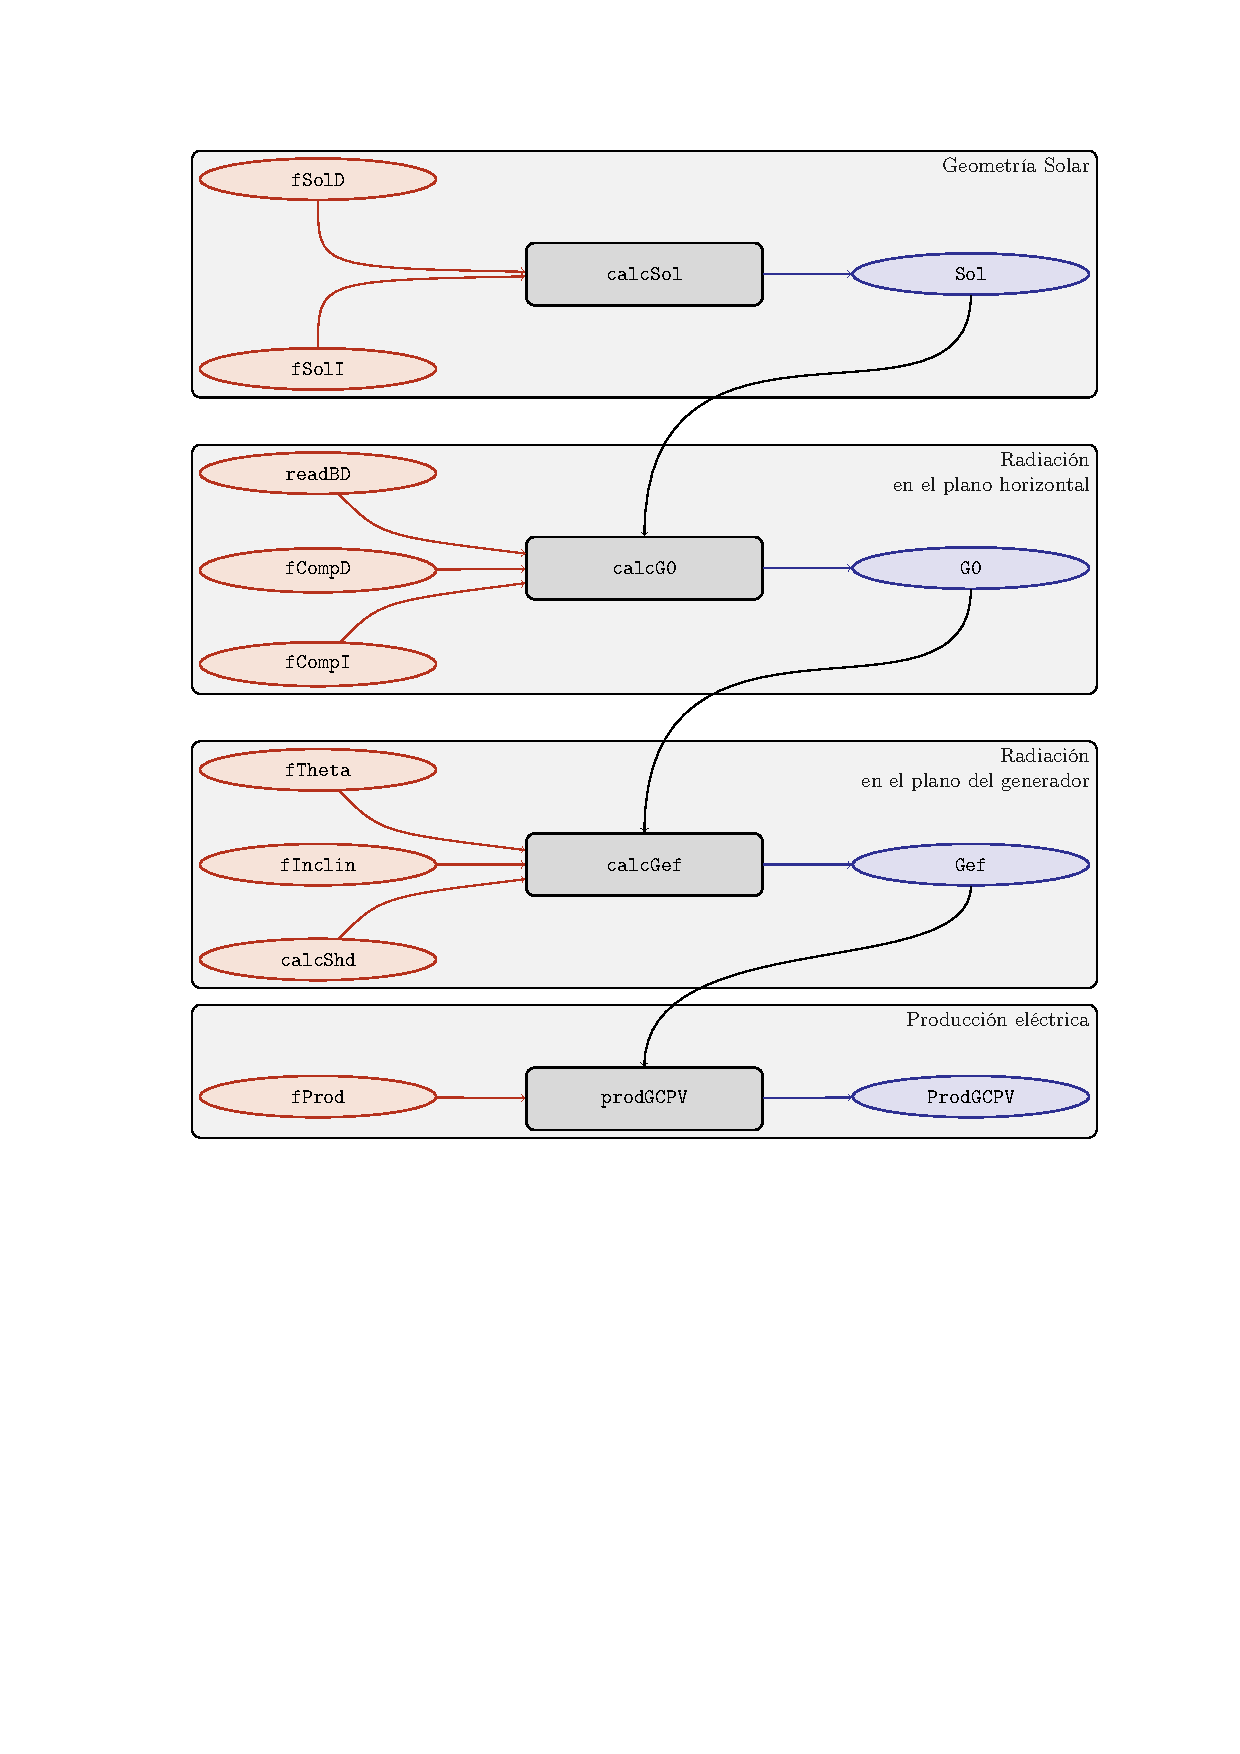
\includegraphics[keepaspectratio,width=0.8\textwidth,height=0.5\textheight]{figuras/procedure.pdf}
\caption{\label{fig:org9ba4490}Proceso de cálculo de las funciones de \texttt{solaR2}}
\end{figure}
A la hora de estimar la producción, el programa sigue los siguientes procesos:
\section{Geometría solar.}
\label{sec:org3065f42}
\label{sec:geometria-solar}
Para calcular la geometría que definen las posiciones de la Tierra y el Sol, \texttt{solaR2} se vale de una función constructora, \texttt{calcSol} [\ref{subsec:calcsol}], la cual mediante las funciones \texttt{fSolD} [\ref{subsec:fsold}] y \texttt{fSolI} [\ref{subsec:fsoli}] cálcula todos los ángulos y componentes que caracterizan la geometría solar.

Como se puede ver en la figura \ref{fig:calcSol}, \texttt{calcSol} funciona gracias a dos funciones:
\begin{itemize}
\item \texttt{fSolD}: la cual computa la geometría a nivel diario, es decir, los ángulos y componentes que se pueden calcular en cada día independiente.
estas son:
\begin{itemize}
\item Declinación (\(\delta\)): calculada a partir de la función \texttt{declination}\footnote{Todas las funciones mencionadas en este punto, se encuentran en el apartado \ref{subsec:utils-angles}.}.
\item Excentricidad (\(\epsilon_o\))
\end{itemize}
\item \texttt{fSolI}: que calcula la geometría a nivel intradiario, es decir, aquella que se puede calcular en unidades infinitesimas de tiempo.
\end{itemize}
\begin{figure}[]
\centering
\includegraphics[keepaspectratio,width=0.8\textwidth,height=0.5\textheight]{figuras/calcSol.pdf}
\caption{Cálculo de la geometría solar mediante la función \texttt{calcSol}, la cual unifica las funciones \texttt{fSolD} y \texttt{fSolI} resultando en un objeto clase \texttt{Sol} el cual contiene toda la información geométrica necesaria para realizar las siguientes estimaciones. \label{fig:calcSol}}
\end{figure}

\subsection{Radiación en el plano horizontal.}
\label{sec:org7322672}
\begin{enumerate}
\item La información de irradiación en el plano horizontal (en todos sus componentes o, en su defecto, solo la global(\(G_d(0)\))) y temperatura viene dada en un objeto de clase \texttt{Meteo}.
\item Mediante la función fCompD, se calcula:
\begin{itemize}
\item La fracción de radiación difusa diaria (\(F_{Dd}\)).
\item El índice de claridad diario (\(K_{Td}\)).
\item Si solo se tienen datos de la componente global de irradición:
\begin{itemize}
\item La irradiación directa en el plano horizontal (\(B_d(0)\)).
\item La irradiación difusa en el plano horizontal (\(D_d(0)\)).
\end{itemize}
\end{itemize}
\item Mediante la función fCompI, se calcula:
\begin{itemize}
\item La fracción de radiación difusa (\(F_D\)).
\item El índice de claridad (\(K_T\)).
\item Si solo se tienen datos de la componenete global de irradiancia (\(G(0)\)):
\begin{itemize}
\item La irradiancia directa en el plano horizontal (\(B(0)\)).
\item La irradiancia difusa en el plano horizontal (\(D(0)\)).
\end{itemize}
\end{itemize}
\item El resultado de ambas funciones junto a medias mensuales y valores anuales se consolidan en un solo objeto de clase \texttt{G0} (que incluye los objetos \texttt{Sol} y \texttt{Meteo} de los que parte) mediante la función calcG0.
\end{enumerate}
\subsection{Radiación en el plano del generador.}
\label{sec:org2443e7d}
\begin{enumerate}
\item La información de radiación puede venir dada en forma de un objeto de clase \texttt{Meteo} o un objeto de clase \texttt{G0} (ya que es este último el que se necesita para estimar la radiación en el plano del generador).
\item Mediante la función fTheta, se calcula:
\begin{itemize}
\item Ángulo de inclinación de la superficie del módulo (\(\beta\)).
\item Ángulo azimutal de la superficie del módulo (\(\alpha\) ).
\item Ángulo de incidencia de la irradiancia solar en la superficie del módulo (\(\theta_s\)).
\end{itemize}
\item Mediante la función fInclin, se calcula:
\begin{itemize}
\item La irradiancia extra-terrestre en la superficie inclinada (\(B_0(\beta, \alpha)\)).
\item La irradiancia directa normal (\(B(n)\)).
\item Las irradiancias global (\(G(\beta, \alpha)\)), directa (\(B(\beta, \alpha)\)), difusa (\(D(\beta, \alpha)\))(total, isotropica y anisotrópica) y del albedo (\(R(\beta, \alpha)\)) sobre una superficie inclinada.
\item Las irradiancias efectivas global (\(G_{ef}(\beta, \alpha)\)), directa (\(B_{ef}(\beta, \alpha)\)), difusa (\(D_{ef}(\beta, \alpha)\))(total, isotropica y anisotrópica) y del albedo (\(R_{ef}(\beta, \alpha)\)) sobre una superficie inclinada.
\item Los factores de pérdidas angulares para las componentes directa (\(FT\)), difusa (\(FT_D\)), y del albedo (\(FT_R\)).
\end{itemize}
\item Mediante la función calcShd, se puede calcular:
\begin{itemize}
\item La irradiancia e irradiación incluyendo sombras para seguidores a dos ejes y horizontales y paneles fijos mediante la función fSombra.
\end{itemize}
\item El resultado de estas funciones junto a medias mensuales y valores anuales se consolidan en un solo objeto de clase \texttt{Gef} (que incluye el objeto \texttt{G0} del que parte) mediante la función calcGef.
\end{enumerate}
\subsection{Producción eléctrica.}
\label{sec:org2f3c838}
\begin{enumerate}
\item Mediante la función fProd, se calcula:
\begin{itemize}
\item La potencia en corriente continua (\(P_{DC}\)).
\item La potencia en corriente alterna (\(P_{AC}\)).
\end{itemize}
\item Estos resultados, llevados a valores diarios, mensuales y anuales, se pueden convertir en valores de energía (\(E_{DC}\) y \(E_{AC}\)) y de productividad del sistema (\(Y_f\)), los cuales se consolidan en un solo objeto de clase \texttt{ProdGCPV} (que incluye el objeto \texttt{Gef} del que parte) mediante la función prodGCPV.
\end{enumerate}
